


\section{Auswertung}
\label{sec:auswertung}

In diesem Kapitel werden die aufgenommenen Messwerte ausgewertet.
\subsection{Vorbereitung}
\label{sec:vorbereitunf}
\subsubsection{Luhmer-Gehrcke Platte}
\label{sec:luhmer}
Die Eigenschaften der Luhmer-Ghercke Platte lassen sich mit den Materialeigenschaften
der Platte bestimmen. Die in diesem Versuch verwendete Luhmer Ghercke Platte hat die
Maße $d=\SI[]{4}[]{mm}$, $L=\SI[]{120}[]{mm}$. Die beiden Spektrallinien welche betrachtet werden sollen
sind:
\begin{center}
  $\lambda_{rot}=\SI[]{643.8}[]{nm}$ und
  $\lambda_{blau}=\SI[]{480.0}[]{nm}$.
\end{center}
Für diesen Versuchsaufbau ergeben sich die Wellenlängenabhängigen Brechungsindizes:
\begin{center}
  $n_{rot}=1.4567$ und
  $n_{blau}=1.4635$.
\end{center}
Mit diesen Angaben kann dann über \autoref{eq:aufloesungsvermoegen} das Auflösungsvermögen $A$ und über
\autoref{eq:dispersionsgebiet} das Dispersionsgebiet $\Delta\lambda$ berechnet werden. Die Ergebnisse
sind in \autoref{tab:LGPlatte} dargestellt.
\begin{table}
  \centering
    \caption{Wellenlängenabhängige Werte der Lummer-Gehrke Platte.}
    \label{tab:LGPlatte}
    \sisetup{table-format=1.2}
    \begin{tabular}{S[table-format=3.2] | S S S [table-format=3.2]}
      \toprule
      {Größe}&{$\SI[]{643.8}[]{nm}$} & {$\SI[]{480.0}[]{nm}$}\\
      \midrule
      {$$A$$}&{$$209128.59$$}&{$$285458.06$$}\\
      {$\Delta \lambda_D / \si[]{\pico\metre} $}&{$$48.91$$}&{$$26.95$$}\\
      \bottomrule
    \end{tabular}
  \end{table}

  \subsubsection{Bestimmung der Landé-Faktoren}
  Die Unterschiede in der Aufspaltung der Spektrallinien ist abhängig von den Landé
Faktoren $g_j$. Für den roten Übergang zwischen den Niveaus $^1 P_1 \leftrightarrow  ^1D_2$ und den blauen
Übergang zwischen den Niveaus $^3 S_1 \leftrightarrow  ^3P_1$ ergeben sich für die einzelnen Landé Faktoren,
mit \autoref{eq:lande} die Werte in \autoref{tab:lande}. Mit der Notation $^{2𝑆+}1𝐿_𝑗$ für die Niveaus, wobei
$L$ der Name des Niveaus ist, welchem ein fester Drehimpuls zugeordnet ist, ergibt sich
\begin{table}
  \centering
    \caption{Berchnung der Landé-Faktoren.}
    \label{tab:lande}
    \sisetup{table-format=1.2}
    \begin{tabular}{S[table-format=3.2] | S S S S S [table-format=3.2]}
      \toprule
      {Niveau}&{J}&{S}&{L}  & {$g_j$}\\
      \midrule
      {$ ^1 P_1$}&{1}&{0}&{1}&{$1$}\\
      {$ ^1 D_2$}&{2}&{0}&{2}&{$1$}\\
      {$ ^3 S_1$}&{1}&{1}&{0}&{$2$}\\
      {$ ^3 P_1$}&{1}&{1}&{1}&{$\frac{2}{2}$}\\
      
      \bottomrule
    \end{tabular}
  \end{table}
  Für die Energiedifferenz zwischen den einzelnen Niveaus ergeben sich nun aus \autoref{eq:nzeeman} 
  folgend die Werte für den normalen Zeeman Effekt in \autoref{tab:normZeemann}.
  \begin{table}
    \centering
      \caption{Berchnung der Landé-Faktoren des normalen Zeemann-Effektes.}
      \label{tab:normZeemann}
      \sisetup{table-format=1.2}
      \begin{tabular}{S[table-format=3.2]  S S S S S [table-format=3.2]}
        \toprule
        {$\SI[]{643.8}[]{\nano \metre}$}&{$$\Delta m =-1$$}&{$$\Delta m =0$$}  & {$$\Delta m =+1$$}\\
        \midrule
        {$ $}&{$\mu_BB$}&{$0$}&{$\mu_BB$}\\
        \bottomrule
      \end{tabular}
    \end{table}
  Für den anormalen Zeeman Effekt können die Faktoren über \autoref{eq:anzeeman} bestimmt werden.
  Sie sind in \autoref{tab:anormZeemann} dargestellt.
    \begin{table}
      \centering
        \caption{Berchnung der Landé-Faktoren des anormalen Zeemann-Effektes.}
        \label{tab:anormZeemann}
        \sisetup{table-format=1.2}
        \begin{tabular}{S[table-format=3.2]  S S S S S [table-format=3.2]}
          \toprule
          {$\SI[]{480.0}[]{\nano \metre}$}&{$$\Delta m =-1$$}&{$$\Delta m =0$$}  & {$$\Delta m =+1$$}\\
          \midrule
          {$ $}&{$\frac{3}{2}\mu_BB$}&{$-\frac{1}{2}\mu_BB$}&{$--BB$}\\
          {$ $}&{$2\mu_BB$}&{$0$}&{$-2\mu_BB$}\\
          {$ $}&{$--$}&{$\frac{1}{2}\mu_BB$}&{$\frac{3}{2}\mu_BB$}\\
          \bottomrule
        \end{tabular}
      \end{table}
\subsubsection{Berechnung der optimalen B-Feldstärken}
Um zu vermeiden das sich Linien überschneiden da sie sich entweder zuweit voneinander entfernen 
oder nicht weit genug, werden hier die optimalen Feldstärken berechnet.
Es ergibt sich über:
\begin{equation}
  B=\frac{hc}{4\mu_B\lambda^2g_{ij}}=\frac{\Delta E}{\mu_B g_{ij}}
\end{equation}
Die sich daraus ergebenden idealen B-Feldstärken sind in \autoref{tab:feldstaerken} dargestellt.
\begin{table}
  \centering
    \caption{Berchnung der Landé-Faktoren des anormalen Zeemann-Effektes.}
    \label{tab:feldstaerken}
    \sisetup{table-format=1.2}
    \begin{tabular}{S[table-format=3.2]  S S S S S [table-format=3.2]}
      \toprule
      {$\Delta g_{ij}$}&{$B$/T}\\
      \midrule
      {$0.5$}&{$1.25$}\\
      {$1.0$}&{$0.63$}\\
      {$1.5$}&{$0.42$}\\
      {$2.0$}&{$0.31$}\\
      \bottomrule
    \end{tabular}
  \end{table}
\subsection{Vermessung des Elektromagneten}
Es ist aufgrund des Versuchsaufbaus nicht möglich die magnetische Flussdichte $B$ zwischen den 
beiden Polschuhen des Elektromagneten zu bestimmen während die Cadmiumdampflampe eingeführt ist.
Daher muss das Magnetfeld vorher mittels einer Hallsonde in abhängigkeit vom Spulenstrom ausgemessen
werden. Wenn die Cadmiumdampflampe dann eingeführt ist muss nurnoch der passende Spulenstrom 
eingestellt werden. In \autoref{tab:magnetfeld} sind die Messdaten für die abfallende Seite der
Hysteresekurve dargestellt.
\begin{table}
    \centering
      \caption{In der Tabelle sind die Messdaten für den Spulenstrom $I$ und die resultierende Flussdichte $B$ dargestellt.}
      \label{tab:magnetfeld}
      \sisetup{table-format=1.2}
      \begin{tabular}{S[table-format=3.2] S S [table-format=3.2]}
        \toprule
        {$I$/[$\si[]{A}$]} & {$B$/[$\si[]{mT}$]}\\
        \midrule
        {$$5.0$$} & {$$ 452.1$$}\\
        {$$4.8$$} & {$$	440.4$$}\\
        {$$4.6$$} & {$$	430.2$$}\\
        {$$4.4$$} & {$$	415.4$$}\\
        {$$4.2$$} & {$$	403.4$$}\\
        {$$4.0$$} & {$$	388.0$$}\\
        {$$3.8$$} & {$$	371.7$$}\\
        {$$3.6$$} & {$$	356.7$$}\\
        {$$3.4$$} & {$$	338.8$$}\\
        {$$3.2$$} & {$$	320.9$$}\\
        {$$3.0$$} & {$$	305.5$$}\\
        {$$2.8$$} & {$$	288.2$$}\\
        {$$2.6$$} & {$$	266.8$$}\\
        {$$2.4$$} & {$$	248.8$$}\\
        {$$2.2$$} & {$$	229.6$$}\\
        {$$2.0$$} & {$$	209.2$$}\\
        {$$1.6$$} & {$$	169.8$$}\\
        {$$1.2$$} & {$$	131.1$$}\\
        {$$0.8$$} & {$$	89.4$$}\\
        {$$0.4$$} & {$$	50.7$$}\\
        {$$0.0$$} & {$$	 9.9$$}\\
        
        \bottomrule
      \end{tabular}
    \end{table}

    Die Daten aus \autoref{tab:magnetfeld} wurden in \autoref{fig:magnetfeld} dargestellt. Zudem wurde 
    an die Daten ein Polynom dritten Grades angepasst die verwendeten Parameter lauten:
    \begin{center}
        $$a_3 = -0.00105 \pm 0.00008$$\\
        $$a_2 =  0.00359 \pm 0.00062$$\\
        $$a_1 =  0.09673 \pm 0.00135$$\\
        $$a_0 =  0.01059 \pm 0.00080$$
        
    \end{center}

    \begin{figure}
        \centering
        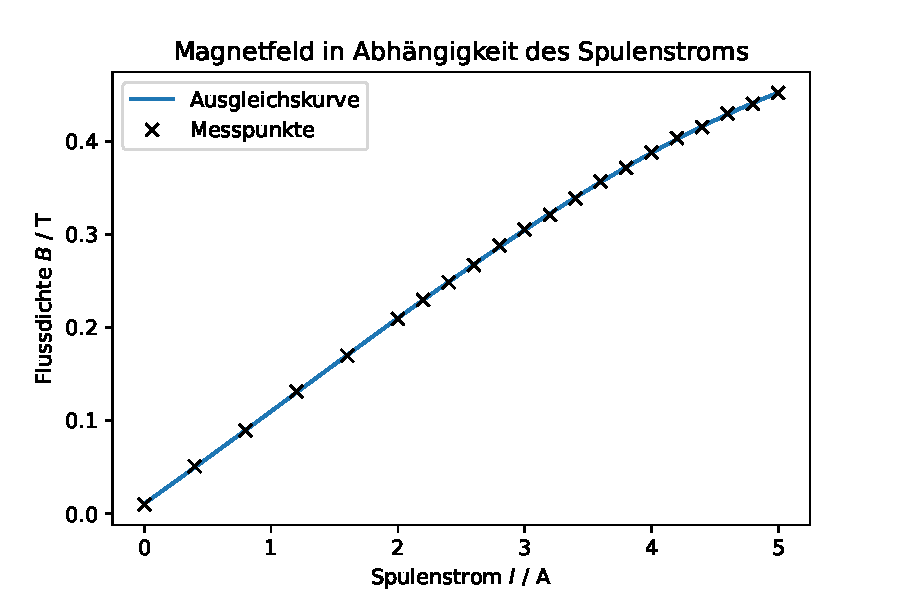
\includegraphics[width=1\textwidth]{content/grafiken/magnetfeld.pdf}
        \caption{Magnetische Flussdichte des verwendeten Elektromagneten in Abhängigkeit des Spulenstroms.}
        \label{fig:magnetfeld}
      \end{figure}
\subsection{Vermessung der Spektrallinien}
\label{sec:linien}
Um die Linien zu vermessen wurde das Licht aus der Lummer-Geehrke Platte mit einer CAD-Kamera
aufgenommen. Anschließend wurde mittels eines Python-Programms jeweils die  vertikal mittlere
Pixelzeile herausgeschnitten und in Graustufen umgerechnet. Die jeweiligen Werte für die Helligkeit wurden 
gegen die Pixelposition aufgetragen, Die jeweiligen Plots sind in \autoref{sec:plots} zu sehen.  Das Programm 
zählte dann die  Pixel welche zwischen zwei Maxima liegen. 
\FloatBarrier
\subsubsection{Die rote Sigma-Linie}

\begin{figure}
  \centering
  
\includegraphics[width=0.75\textwidth]{content/grafiken/rot 0.JPG}
  \caption{Die rote Spektrallienie, oben ohne Magnetfeld, unten mit Magnetfeld.}
  \label{fig:rot0}
\end{figure}

Diese Daten sind mit der zugehörigen Wellenlängenverschiebung
$\delta \lambda$ in \autoref{tab:ergebnisse1} dargestellt. Die Wellenlängenverschiebung berechnet sich über:
\begin{equation}
  \delta \lambda =\frac{\delta s}{2\delta S}\Delta \lambda_D
\end{equation}
\begin{table}
\centering
\caption{Wellenlängenverschiebung der roten Sigma-Linie.}
\label{tab:tabelleRot}
\sisetup{table-format=1.2}
\begin{tabular}{S[table-format=3.2] S S S [table-format=3.2]}
\toprule
{Mode Nr.} & {$\Delta S$/px}&{$\delta S$ /px}&{$\delta \lambda$ /pm}\\
\midrule
{$$0$$}&{$$119$$}&{$$37$$}&{$$7.6$$}\\
{$$1$$}&{$$124$$}&{$$31$$}&{$$6.11$$}\\
{$$2$$}&{$$124$$}&{$$41$$}&{$$8.09$$}\\
{$$3$$}&{$$133$$}&{$$52$$}&{$$9.56$$}\\
{$$4$$}&{$$134$$}&{$$47$$}&{$$8.58$$}\\
{$$5$$}&{$$145$$}&{$$53$$}&{$$8.94$$}\\
{$$7$$}&{$$149$$}&{$$44$$}&{$$7.22$$}\\
{$$8$$}&{$$160$$}&{$$56$$}&{$$8.56$$}\\
{$$9$$}&{$$165$$}&{$$48$$}&{$$7.11$$}\\
{$$10$$}&{$$180$$}&{$$71$$}&{$$9.65$$}\\
{$$11$$}&{$$196$$}&{$$81$$}&{$$10.11$$}\\
{$$12$$}&{$$218$$}&{$$75$$}&{$$8.41$$}\\
\midrule
{$$\diameter$$}&{$$$$}&{$$$$}&{$$8.33\pm0.34$$}\\
\bottomrule
\end{tabular}
\end{table}

Aus diesen Daten wurde dann jeweils ein Mittelwert nach \autoref{eq:Mittelwert} mit zugehörigem Fehler nach
\autoref{eq:mittelwertfehler} berechent.

\FloatBarrier
\newpage
\subsubsection{Die blaue Pi-Linie}
\begin{figure}
  \centering
  
\includegraphics[width=0.75\textwidth]{content/grafiken/blau 90.JPG}
  \caption{Die Pi-Linie, oben ohne Magnetfeld, unten mit Magnetfeld.}
  \label{fig:blau90}
\end{figure}
\begin{table}
\centering
\caption{Wellenlängenverschiebung der blauen Sigma-Linie.}
\label{tab:tabelleBlau}
\sisetup{table-format=1.2}
\begin{tabular}{S[table-format=3.2] S S S [table-format=3.2]}
\toprule
{Mode Nr.} & {$\Delta S$/px}&{$\delta S$ /px}&{$\delta \lambda$ /pm}\\
\midrule
{$$0$$}&{$$33$$}&{$$22$$}&{$$8.98$$}\\
{$$1$$}&{$$35$$}&{$$12$$}&{$$4.62$$}\\
{$$2$$}&{$$2$$}&{$$4$$}&{$$26.95$$}\\
{$$3$$}&{$$34$$}&{$$24$$}&{$$9.51$$}\\
{$$4$$}&{$$35$$}&{$$23$$}&{$$8.86$$}\\
{$$5$$}&{$$36$$}&{$$22$$}&{$$8.23$$}\\
{$$6$$}&{$$37$$}&{$$16$$}&{$$5.83$$}\\
{$$8$$}&{$$36$$}&{$$6$$}&{$$2.25$$}\\
{$$9$$}&{$$4$$}&{$$23$$}&{$$77.48$$}\\
{$$10$$}&{$$33$$}&{$$4$$}&{$$1.63$$}\\
{$$11$$}&{$$36$$}&{$$18$$}&{$$6.74$$}\\
{$$12$$}&{$$3$$}&{$$4$$}&{$$17.97$$}\\
{$$13$$}&{$$34$$}&{$$21$$}&{$$8.32$$}\\
\midrule
{$$\diameter$$}&{$$$$}&{$$$$}&{$$9.16\pm2.02$$}\\
\bottomrule
\end{tabular}
\end{table}



\FloatBarrier
\newpage
\subsubsection{Die blaue Sigma-Linie}
\begin{figure}
  \centering
  
\includegraphics[width=0.75\textwidth]{content/grafiken/blau 90.JPG}
  \caption{Die blaue Sigma-Lienie, oben ohne Magnetfeld, unten mit Magnetfeld.}
  \label{fig:blau0}
\end{figure}
\begin{table}
\centering
\caption{Wellenlängenverschiebung der blauen Pi-Linie.}
\label{tab:tabelleBlau2}
\sisetup{table-format=1.2}
\begin{tabular}{S[table-format=3.2] S S S [table-format=3.2]}
\toprule
{Mode Nr.} & {$\Delta S$/px}&{$\delta S$ /px}&{$\delta \lambda$}\\
\midrule
{$$0$$}&{$$38$$}&{$$39$$}&{$$19.97$$}\\
{$$1$$}&{$$38$$}&{$$37$$}&{$$18.9458$$}\\
{$$2$$}&{$$39$$}&{$$36$$}&{$$18.9189$$}\\
{$$4$$}&{$$39$$}&{$$36$$}&{$$18.9189$$}\\
{$$5$$}&{$$35$$}&{$$38$$}&{$$17.9218$$}\\
\midrule
{$$\diameter$$}&{$$$$}&{$$$$}&{$$18.94\pm0.32$$}\\
\bottomrule
\end{tabular}
\end{table}



\FloatBarrier
\newpage
\subsection{Bestimmung der Lanndé-Faktoren}
Um die Landé Faktoren zu bestimmen, wird von der Formel für die Veränderung der
Energie \autoref{eq:anzeeman} ausgegangen:
\begin{equation*}
  \Delta E = g_{ij} \mu_B B m_J\\
  \Leftrightarrow g_{ij}=\frac{\Delta E}{\mu_B B} 
\end{equation*}
$\mu_B$ ist dabei das Bohrsche Magneton und $g=g_{ij}$ der gewünschte Landé Faktor, nach
dem direkt umgestellt wurde. In erster Näherung
\begin{equation*}
  \Delta E=E(\lambda+\delta \lambda) - E(\lambda)
\end{equation*}
ergibt die Taylorentwicklung:
\begin{equation*}
  \Delta E=\frac{\delta E}{\delta \lambda} E(\lambda).
\end{equation*}
Diese wird mit der quantenmechanischen Energie $E(\lambda)=\frac{hc}{\lambda }$
in den Landé Faktor eingesetzt und es folgt:
\begin{equation*}
  g=\frac{\delta \lambda hc}{\mu_B B \lambda^2}
\end{equation*}
Nun können mithilfe der in \autoref{sec:linien} bestimmten Wellenlängenverschiebungen die
Landé-Faktoren berechnet werden.


\begin{table}
  \centering
    \caption{Die berechneten Landé-Faktoren}
    \sisetup{table-format=1.2}
    \begin{tabular}{S[table-format=3.2] S S S S [table-format=3.2]}
      \toprule
      {$\lambda/\si[]{\nano \metre}$} &{Übergang} & {$\delta \lambda / \si[]{\pico \metre}$}&{$g_{j}$}\\
      \midrule
      {$648.8$}&{$\sigma$}&{$209.24\pm 29.86$}&{$23.5504\pm $}\\
      {$480.0$}&{$\sigma$}&{$8.89\pm 0.7$}&{$2.3817\pm $}\\
      {$480.0$}&{$\pi$}&{$21.34\pm 0.44 $}&{$4.3882\pm $}\\
      \bottomrule
    \end{tabular}
  \end{table}












  \subsection{Helligkeitsplots}
\label{sec:plots}
\twocolumn[]
      
      \newpage
      \begin{figure}
        \centering
        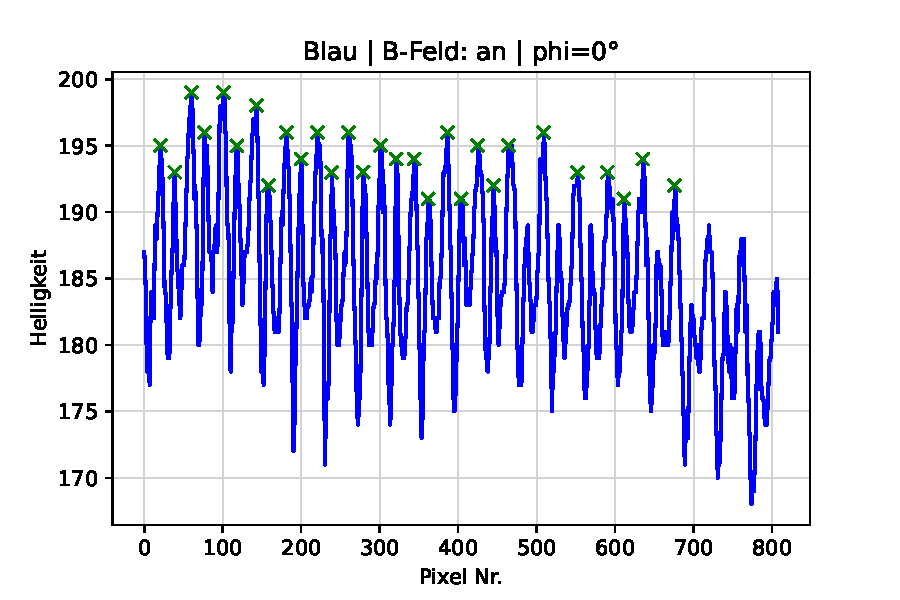
\includegraphics[width=0.5\textwidth]{content/grafiken/blau mit magnet 0 gimbplot.pdf}
        \caption{}
        \label{fig:bmm0}
      \end{figure}
      
      \begin{figure}
        \centering
        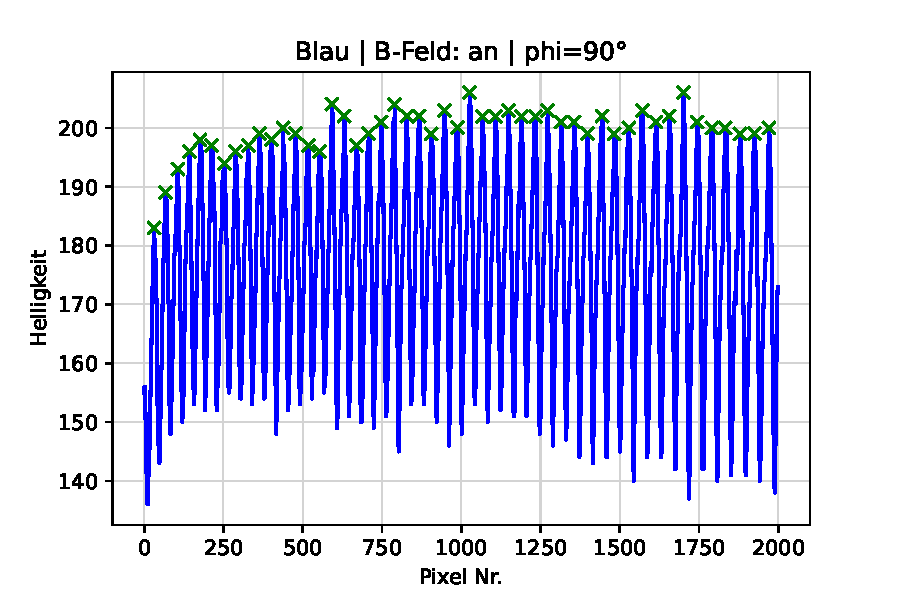
\includegraphics[width=0.5\textwidth]{content/grafiken/blau mit magnet 90 gimbplot.pdf}
        \caption{}
        \label{fig:bmm90}
      \end{figure}
      
      \begin{figure}
        \centering
        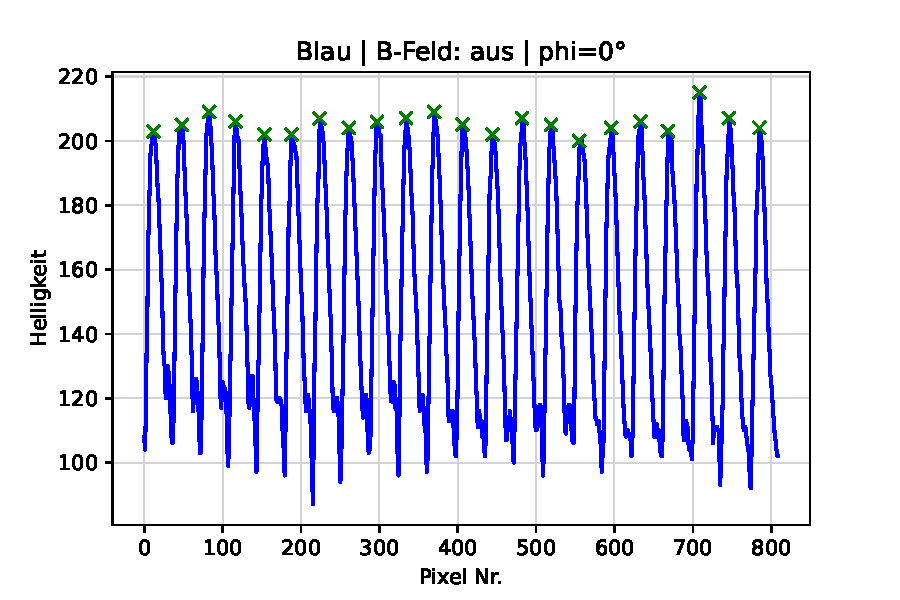
\includegraphics[width=0.5\textwidth]{content/grafiken/blau ohne magnet 0 gimbplot.pdf}
        \caption{}
        \label{fig:bom0}
      \end{figure}
      
      \begin{figure}
        \centering
        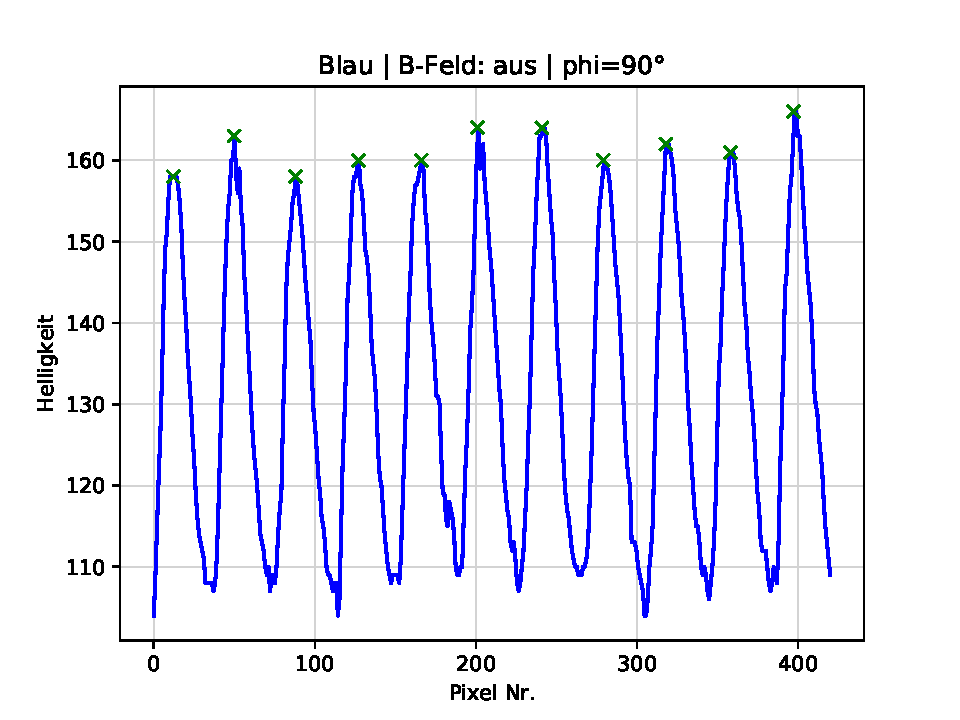
\includegraphics[width=0.5\textwidth]{content/grafiken/blau ohne magnet 90 gimbplot.pdf}
        \caption{}
        \label{fig:bom90}
      \end{figure}
      
      \begin{figure}
        \centering
        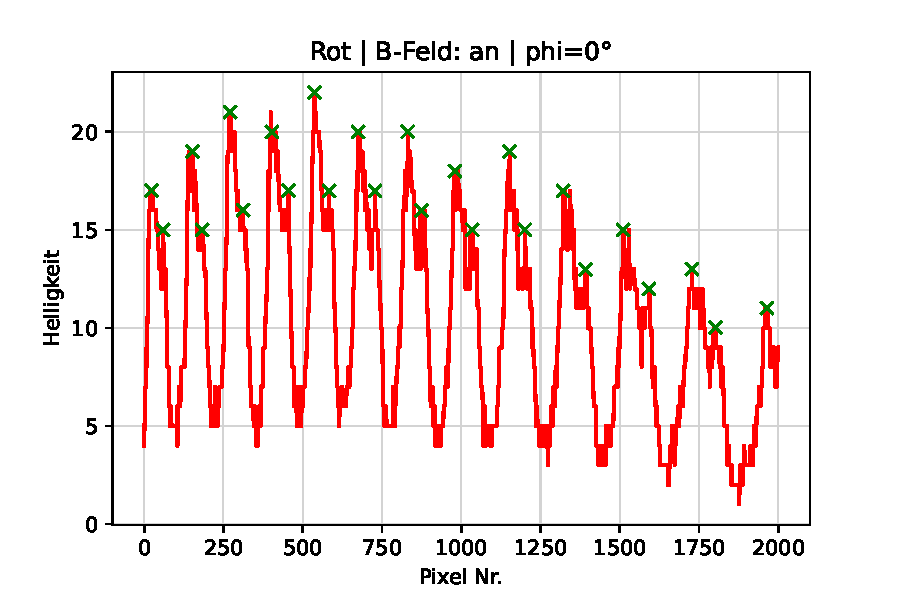
\includegraphics[width=0.5\textwidth]{content/grafiken/rot mit magnet 0 gimbplot.pdf}
        \caption{}
        \label{fig:rmm0}
      \end{figure}
      
      \begin{figure}
        \centering
        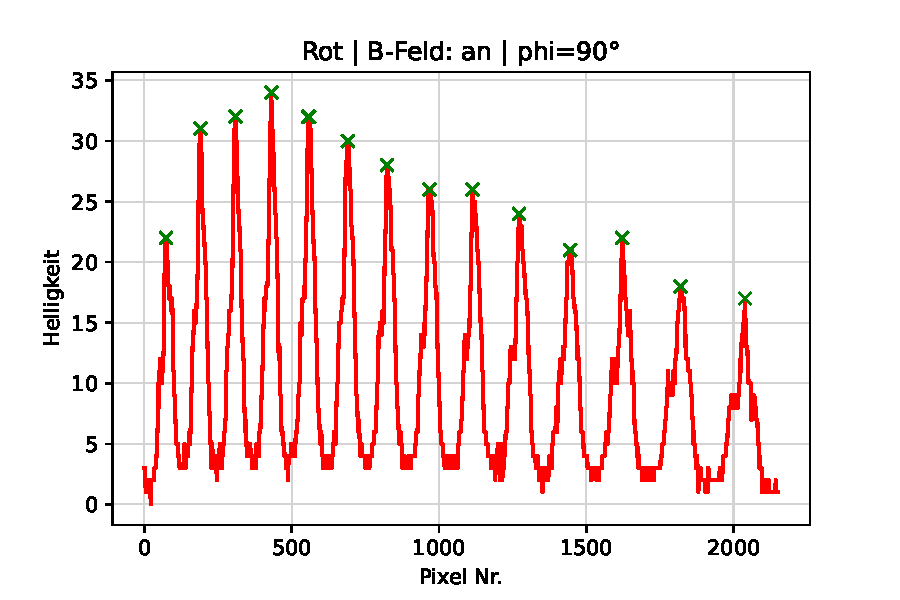
\includegraphics[width=0.5\textwidth]{content/grafiken/rot mit magnet 90 gimbplot.pdf}
        \caption{}
        \label{fig:rmm90}
      \end{figure}
      
      \begin{figure}
        \centering
        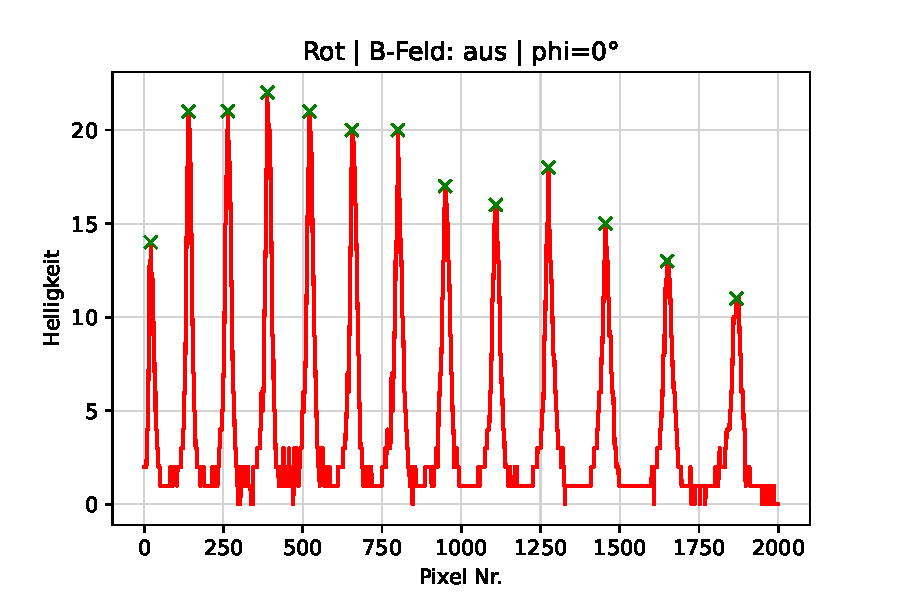
\includegraphics[width=0.5\textwidth]{content/grafiken/rot ohne magnet 0 gimbplot.pdf}
        \caption{}
        \label{fig:rom0}
      \end{figure}
      
      \begin{figure}
        \centering
        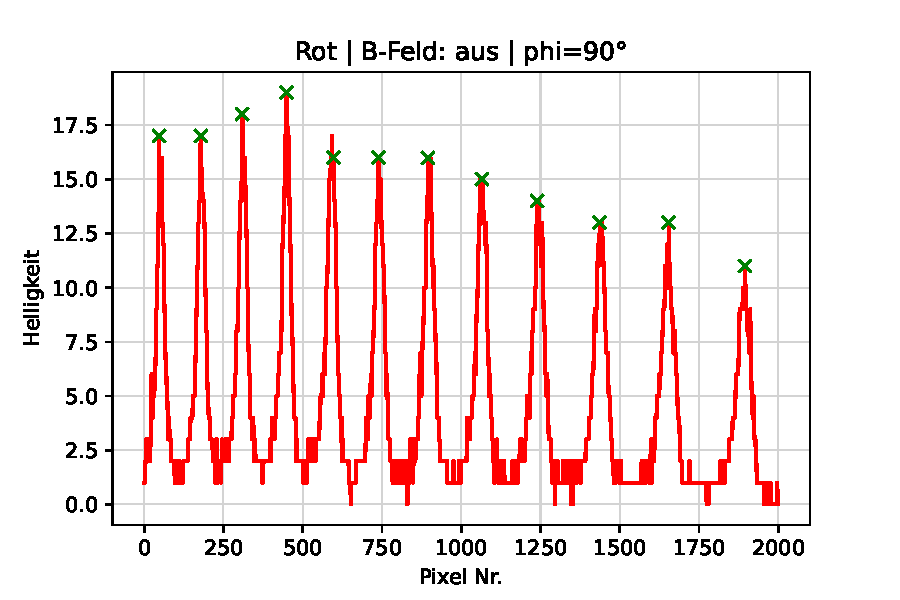
\includegraphics[width=0.5\textwidth]{content/grafiken/rot ohne magnet 90 gimbplot.pdf}
        \caption{}
        \label{fig:rom90}
      \end{figure}
\onecolumn

